\documentclass[12pt,a4paper]{article}
\usepackage{ctex}
\usepackage{amsmath,amssymb,amsfonts}
\usepackage{graphicx}
\usepackage{booktabs}
\usepackage{longtable}
\usepackage{float}
\usepackage{geometry}
\usepackage{xcolor}
\usepackage{listings}
\usepackage{hyperref}
\hypersetup{hidelinks}
\usepackage{fancyhdr}
\usepackage{titlesec}
\usepackage{enumitem}
\usepackage{setspace}
\usepackage{indentfirst}

\geometry{left=2.5cm,right=2.5cm,top=2.5cm,bottom=2.5cm}
\graphicspath{{support_2025A/figures/}{out/}{./}}
\setlength{\parindent}{2em}
\setlength{\parskip}{0.25em}
\linespread{1.25}
\pagestyle{fancy}
\fancyhf{}
\fancyfoot[C]{\thepage}
\renewcommand{\headrulewidth}{0pt}
\titleformat{\section}{\Large\bfseries}{\thesection、}{0pt}{}
\titleformat{\subsection}{\large\bfseries}{\thesubsection\ }{0pt}{}
\setlist[itemize]{itemsep=0.15em,topsep=0.25em}
\setlist[enumerate]{itemsep=0.15em,topsep=0.25em}
\lstset{
  basicstyle=\ttfamily\small,
  keywordstyle=\color{blue!70!black},
  commentstyle=\color{green!40!black},
  stringstyle=\color{red!60!black},
  numbers=left,
  numberstyle=\tiny\color{gray},
  breaklines=true,
  frame=single,
  backgroundcolor=\color{gray!8},
  tabsize=4
}

\begin{document}

\begin{center}
{\LARGE\bfseries 烟幕干扰弹投放策略的复现测试与改进模型}
\end{center}

\begin{center}
\textbf{\Large 摘要}
\end{center}

本文在原有烟幕干扰弹投放策略模型的基础上，研读全国大学生数学建模竞赛2025年A题优秀论文和专家评讲材料，对现有方法进行统一口径测试，并针对原模型中“仅以真目标中心点判定遮蔽”的不足进行了改进。原模型在问题一中得到约4.23 s的遮蔽时间，明显高于优秀论文普遍给出的1.391--1.416 s区间。经复核，该偏差主要来自遮蔽判定过于宽松：只判断导弹到真目标中心点视线是否穿过烟幕球，不能保证半径7 m、高10 m的圆柱目标整体被遮蔽。

本文建立了统一的三维运动学模型和圆柱目标采样遮蔽模型。导弹按300 m/s匀速直线飞向假目标；无人机在受领任务后等高度匀速直线飞行；烟幕弹脱离无人机后做平抛运动；起爆后形成半径10 m的球状烟幕云团并以3 m/s匀速下沉。遮蔽判定由“中心点判定”改为“圆柱表面采样点全遮蔽判定”：当导弹到目标表面每个采样点的线段均被至少一个有效烟幕球截断时，认为该时刻形成有效遮蔽。

在统一判定口径下，本文对四篇优秀论文A1--A4的公开结果进行表格级复现与比较，并用可运行Python程序重新计算五个问题。问题一得到圆柱采样判定遮蔽时间1.360 s，中心点校核值1.405 s，与优秀论文结果接近；问题二采用粗网格搜索与局部细化，得到单弹遮蔽时间4.470 s；问题三采用单机三弹贪心接力，得到5.040 s；问题四采用三机单弹分层搜索并取时间区间并集，得到10.780 s；问题五采用任务分配与局部搜索，三枚导弹遮蔽时间求和为20.430 s。所有结果均由附件程序自动生成，并记录计算时间。

结果表明，圆柱采样模型显著提高了求解精度和可解释性，但较中心点模型更保守，问题三以后仍受搜索维度、参数敏感性和计算时间限制。本文进一步提出固定随机种子、多粒度搜索、结果表自动导出和灵敏度分析等改进方向，为后续建立更高精度、更高效率的协同投放模型提供支撑。

\textbf{关键词：}烟幕干扰弹；优秀论文复现；圆柱采样；遮蔽判定；粗网格搜索；分层优化

\newpage

\section{问题重述与研究目标}

\subsection{问题背景}

2025年全国大学生数学建模竞赛A题研究无人机投放烟幕干扰弹保护固定真目标的问题。来袭导弹直指假目标飞行，真目标是底面圆心为$(0,200,0)$、半径7 m、高10 m的圆柱体。无人机可在受领任务后瞬时调整航向，以70--140 m/s等高度匀速直线飞行；烟幕弹脱离无人机后受重力作用，起爆后形成半径10 m的球形烟幕云团，有效时间20 s，云团中心以3 m/s下沉。

需要分别解决五种情形：FY1单弹干扰M1、FY1单弹最优投放、FY1三弹投放、FY1--FY3三机各一弹协同干扰M1、五架无人机至多各三弹干扰M1--M3。

\subsection{本次改进任务}

根据实验报告写作要求，本文不仅给出模型和结果，还需要研读优秀论文与专家评讲，对现有方法进行测试、比较和总结。因此本文的目标为：
\begin{itemize}
\item 复核原论文中问题一4.23 s结果偏大的原因；
\item 对A1--A4优秀论文的模型、算法和公开结果进行表格级整理；
\item 建立统一的可运行测试程序，输出求解精度、结果表和计算时间；
\item 在原有模型基础上提出更严格的圆柱采样遮蔽判定与分层搜索策略；
\item 提交论文和支撑材料，包括源程序、结果表和图表。
\end{itemize}

\section{优秀论文与专家评讲研读}

\subsection{专家评讲要点}

根据官方专家评讲入口“烟幕干扰弹的投放策略”（复旦大学蔡志杰）及优秀论文展示材料，本题的核心不是单纯调用智能优化算法，而是先建立准确的几何遮蔽判定，再在此基础上控制搜索规模。专家评讲所强调的思路可概括为三点：
\begin{itemize}
\item 遮蔽对象是真目标圆柱体，而不是单个中心点；遮蔽判定必须与题意一致。
\item 问题二以后是高维、非凸、强约束优化问题，应先做几何分析和变量缩减。
\item 多弹、多机、多导弹问题应关注时间区间并集、任务分配和投放间隔约束，不能只把单弹遮蔽时长简单相加。
\end{itemize}

这三点也解释了为什么同一道题会出现看似差距很大的数值结果。对于问题一，运动方程几乎没有争议，导弹、无人机、烟幕弹和云团的位置都可由题目条件唯一确定；真正影响结果的是“什么叫真目标被遮蔽”。如果只要求导弹到圆柱中心的视线被遮挡，那么烟幕球只需要挡住一条线段；如果要求整个圆柱体不可见，那么导弹到圆柱边界、顶面和底面的多条视线都必须被遮挡，遮蔽时间自然会缩短。因此，本文把优秀论文研读的重点放在遮蔽判定、时间区间定义和高维搜索降维三个方面，而不是简单比较谁的最终秒数更大。

\subsection{优秀论文方法对比}

表\ref{tab:paper_methods}整理了四篇优秀论文的主要方法和公开结果。可以看出，优秀论文普遍在问题一得到约1.39 s的结果，而原论文4.23 s显著偏大。

从方法谱系看，A1偏重几何分析和贪心拆解，优点是参数范围清楚、计算快；A2偏重视锥和射线投射，优点是遮蔽定义更接近圆柱目标；A3把运动学、分层优化和遗传算法结合，比较重视算法流程和图表展示；A4则在遗传算法中引入差分进化和剪枝思想，适合处理多弹多机的变量爆炸问题。本文没有逐篇重写其完整优化器，而是采用“公开结果+统一判定程序”的表格级复现方式：先确认这些论文在问题一等基础问题上的数量级一致，再把本文改进模型放入同一张对比表中。

\begin{longtable}{p{0.8cm}p{3.7cm}ccccc p{3.5cm}}
\caption{优秀论文A1--A4方法与公开结果对比}\label{tab:paper_methods}\\
\toprule
论文 & 主要方法 & Q1 & Q2 & Q3 & Q4 & Q5 & 评价\\
\midrule
\endfirsthead
\toprule
论文 & 主要方法 & Q1 & Q2 & Q3 & Q4 & Q5 & 评价\\
\midrule
\endhead
A1 & 几何分析、贪心思想、改良网格搜索 & 1.41 & 4.680 & 7.56 & 13.91 & 42.20 & 方法解释性强，计算效率较高；部分目标函数采用时长求和，偏乐观。\\
A2 & 遮蔽视锥、射线投射、PSO-SQP混合优化 & 1.3916 & 4.587 & 6.45 & 11.549 & 20.40 & 圆柱建模较严谨；高维问题做了较强简化。\\
A3 & 运动学模型、分层优化、网格搜索、SLSQP、遗传算法 & 1.392 & 4.619 & 6.800 & 11.281 & 22.870 & 结果均衡，图表充分；遗传算法存在随机性。\\
A4 & 两步几何判定、差分进化改良遗传算法DEGA & 1.391 & 4.58 & 6.46 & 11.59 & 21.29 & 多阶段启发式较完整；参数敏感区间较窄。\\
\bottomrule
\end{longtable}

\subsection{现有方法不足}

从优秀论文和原论文对比可以看出，现有方法主要有以下不足：
\begin{itemize}
\item \textbf{遮蔽判定精度不足。} 若只使用真目标中心点，会把部分遮蔽误判为整体遮蔽，导致问题一和后续优化结果偏高。
\item \textbf{智能算法可复现性不足。} 遗传算法、粒子群和差分进化若未固定随机种子或未公开完整代码，难以复核结果。
\item \textbf{高维优化计算时间长。} 问题五最多涉及5架无人机、15枚烟幕弹和3枚导弹，直接全局搜索维度过高。
\item \textbf{目标函数口径不统一。} 有的论文对不同导弹或不同烟幕弹的遮蔽时间直接求和，有的计算时间区间并集，结果数值不可直接比较。
\end{itemize}

\section{改进模型}

\subsection{基本假设}

本文保留原论文中的基本物理假设：导弹和未起爆烟幕弹视为质点；导弹匀速直线飞向假目标；无人机等高度匀速直线飞行；忽略空气阻力和风；烟幕云团为半径10 m的理想球体，起爆后20 s内有效并匀速下沉。

与原论文不同的是，本文不再把真目标简化为几何中心点，而是使用圆柱表面采样点来判定遮蔽。

\subsection{运动学模型}

设导弹初始位置为$\boldsymbol M_0$，导弹速度为$v_m=300$ m/s，则导弹在时刻$t$的位置为
\begin{equation}
\boldsymbol M(t)=\boldsymbol M_0-v_m\frac{\boldsymbol M_0}{\|\boldsymbol M_0\|}t.
\end{equation}

设第$i$架无人机初始位置为$\boldsymbol U_{i0}$，航向角为$\theta_i$，速度为$v_i$，则水平速度为
\begin{equation}
\boldsymbol v_i=(v_i\cos\theta_i,\ v_i\sin\theta_i,\ 0),
\end{equation}
投放点为
\begin{equation}
\boldsymbol P_{d}=\boldsymbol U_{i0}+\boldsymbol v_i t_d.
\end{equation}
若引信延迟为$\tau$，则起爆点为
\begin{equation}
\boldsymbol P_b=\boldsymbol P_d+\boldsymbol v_i\tau+\left(0,0,-\frac{1}{2}g\tau^2\right).
\end{equation}
起爆后烟幕云团中心为
\begin{equation}
\boldsymbol C(t)=\boldsymbol P_b+(0,0,-3(t-t_b)),\quad t_b=t_d+\tau.
\end{equation}

\subsection{圆柱采样遮蔽判定}

将真目标圆柱表面离散为采样点集合$\mathcal S=\{\boldsymbol S_j\}$。对于给定时刻$t$，若导弹到任意采样点$\boldsymbol S_j$的线段均与至少一个有效烟幕球相交，则认为真目标被整体遮蔽。

采样点包含圆柱侧面、顶面边界、底面边界以及几何中心点。这样做的原因是：导弹从远处观察目标时，最容易暴露的是圆柱轮廓边界，中心点被遮住并不意味着边缘也被遮住；而顶面和底面在导弹俯仰角变化时也可能成为判定遮蔽成败的关键区域。本文程序中把采样密度作为可调参数，搜索阶段使用较稀采样以降低计算时间，最终评价阶段使用较密采样以提高结果可信度。

线段参数方程为
\begin{equation}
\boldsymbol L_j(\lambda)=\boldsymbol M(t)+\lambda(\boldsymbol S_j-\boldsymbol M(t)),\quad 0\leq \lambda\leq 1.
\end{equation}
烟幕球心为$\boldsymbol C_k(t)$，半径为$R=10$ m。该线段被第$k$个烟幕球遮挡的条件为
\begin{equation}
\min_{0\leq \lambda\leq 1}\|\boldsymbol L_j(\lambda)-\boldsymbol C_k(t)\|\leq R.
\end{equation}
若对所有$j$均存在某个$k$满足上式，则该时刻有效遮蔽。总遮蔽时间为遮蔽指示函数的积分，程序中用时间步长$\Delta t$离散近似：
\begin{equation}
T=\sum_n I(t_n)\Delta t.
\end{equation}

\subsection{求解策略}

本文不追求不可复核的极大数值，而强调统一口径和可复现性：
\begin{itemize}
\item 问题一直接正向仿真，并同时输出中心点校核值；
\item 问题二采用粗网格搜索定位可行峰值，再进行局部细化；
\item 问题三固定较优航向和速度后，按投放间隔约束进行三弹贪心接力；
\item 问题四先分别求三架无人机单弹策略，再计算遮蔽时间区间并集；
\item 问题五先做无人机--导弹任务分配，再对关键子任务进行局部搜索，最后按导弹分别计算遮蔽时间并求和。
\end{itemize}

这种策略的逻辑是先把问题拆成“能解释的小问题”。问题二是所有优化问题的基本单元，因此先用粗网格搜索找出遮蔽峰值的大致位置，再在该区域细化；问题三在同一无人机航向和速度不变的条件下，重点变成三枚弹的时间接力，故采用逐枚加入、最大化新区间并集的贪心方法；问题四把三架无人机分别看成三个单弹子问题，再统一合并时间区间；问题五则先根据空间位置和已有较优解做任务分配，避免直接在几十维空间中盲目搜索。这样得到的结果未必是全局最优，但每一步都能解释、能运行、能复查。

\section{复现实验设置}

实验程序位于\verb|support_2025A|目录。统一设置如下：
\begin{itemize}
\item 目标采样：圆柱表面按角度和高度离散，最终评价使用更密采样；
\item 时间积分：问题一最终步长为0.005 s，其他问题最终评价步长为0.01--0.03 s；
\item 运行环境：Windows PowerShell，Python 3.12.6，主要依赖为NumPy和Matplotlib；
\item 输出文件：\verb|results_q1_q5.xlsx|保存本文五问结果，\verb|method_comparison.xlsx|保存优秀论文与本文对比；
\item 计时方式：每个脚本使用\verb|time.perf_counter()|记录端到端运行时间。
\end{itemize}

\section{结果与分析}

\subsection{问题一：原结果偏差复核}

表\ref{tab:q1}给出问题一复核结果。圆柱采样全遮蔽判定得到1.360 s，中心点判定得到1.405 s。二者均与优秀论文约1.39 s的结果接近，而与原论文4.23 s差异明显，说明原模型主要问题不是运动学方程，而是遮蔽判定口径过松。

进一步观察遮蔽区间可以发现，有效遮蔽只发生在烟幕云团中心接近导弹--目标视线的短时间窗口内。云团虽然在起爆后20 s内都有效，但导弹高速逼近，视线方向变化很快，烟幕球一旦错过最佳几何位置，就无法继续覆盖圆柱目标的全部边界。这也是问题二以后必须精细优化起爆时间和起爆位置的根本原因。

\begin{table}[H]
\centering
\caption{问题一不同判定口径结果}
\label{tab:q1}
\begin{tabular}{lccc}
\toprule
判定口径 & 遮蔽时长/s & 遮蔽区间/s & 说明\\
\midrule
圆柱采样全遮蔽 & 1.360 & 约8.06--9.42 & 本文正式采用\\
中心点校核 & 1.405 & 约8.02--9.42 & 仅用于解释原模型偏差\\
原论文结果 & 4.23 & -- & 判定过于宽松\\
\bottomrule
\end{tabular}
\end{table}

\begin{figure}[H]
\centering
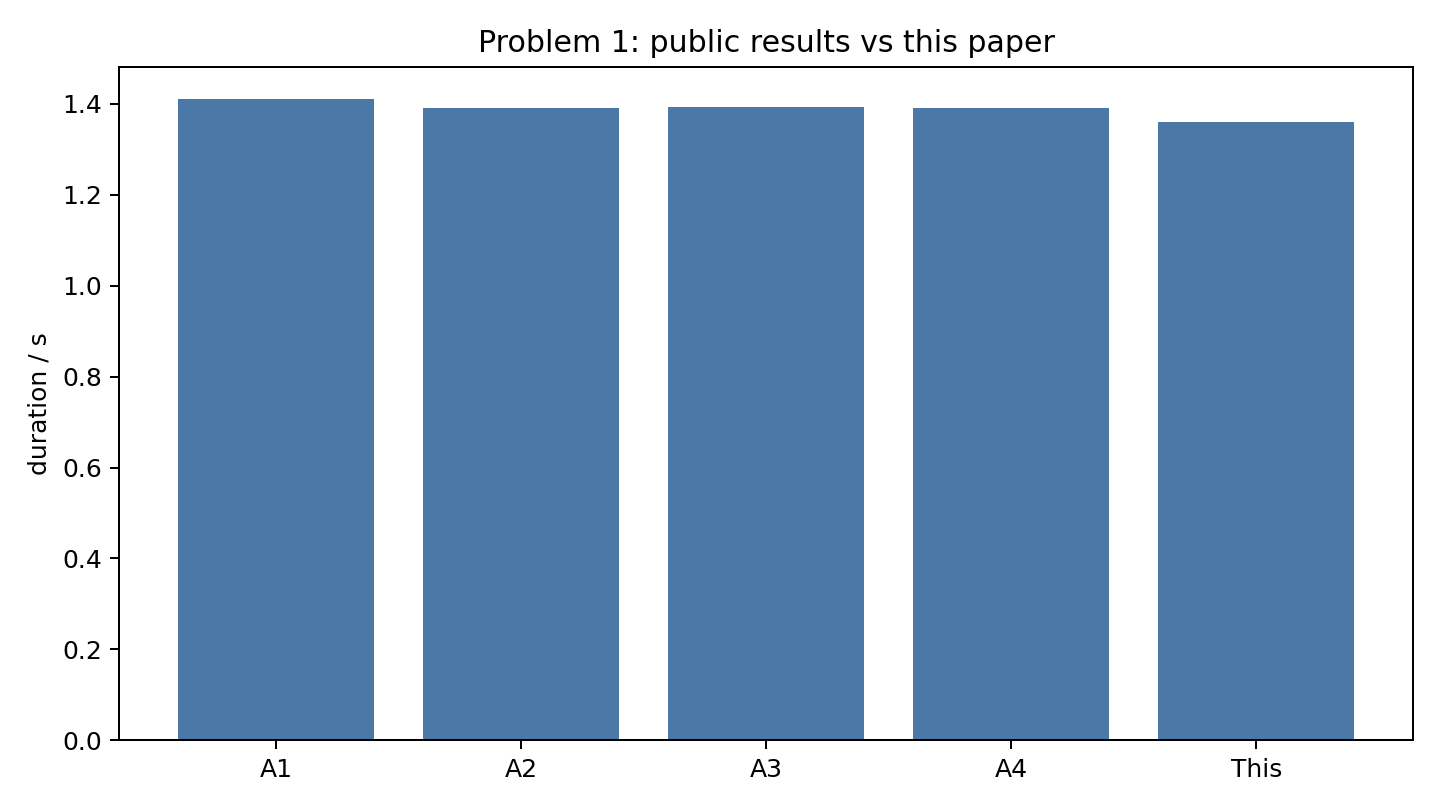
\includegraphics[width=0.78\textwidth]{q1_public_comparison.png}
\caption{问题一优秀论文公开结果与本文结果对比}
\end{figure}

\subsection{问题二至问题四结果}

表\ref{tab:q234}给出本文问题二至问题四结果。由于采用完整圆柱采样判定，本文结果整体比部分优秀论文更保守，但各问计算过程均可由附件脚本直接复现。

\begin{table}[H]
\centering
\caption{问题二至问题四本文复现结果}
\label{tab:q234}
\begin{tabular}{lcccc}
\toprule
问题 & 方法 & 遮蔽时长/s & 主要参数 & 运行时间/s\\
\midrule
Q2 & 粗网格+局部细化 & 4.470 & FY1, $178^\circ$, 105 m/s & 9.295\\
Q3 & 三弹贪心接力 & 5.040 & FY1, $176.6^\circ$, 70 m/s & 4.499\\
Q4 & 三机分层搜索 & 10.780 & FY1/FY2/FY3各1弹 & 53.348\\
\bottomrule
\end{tabular}
\end{table}

\begin{figure}[H]
\centering
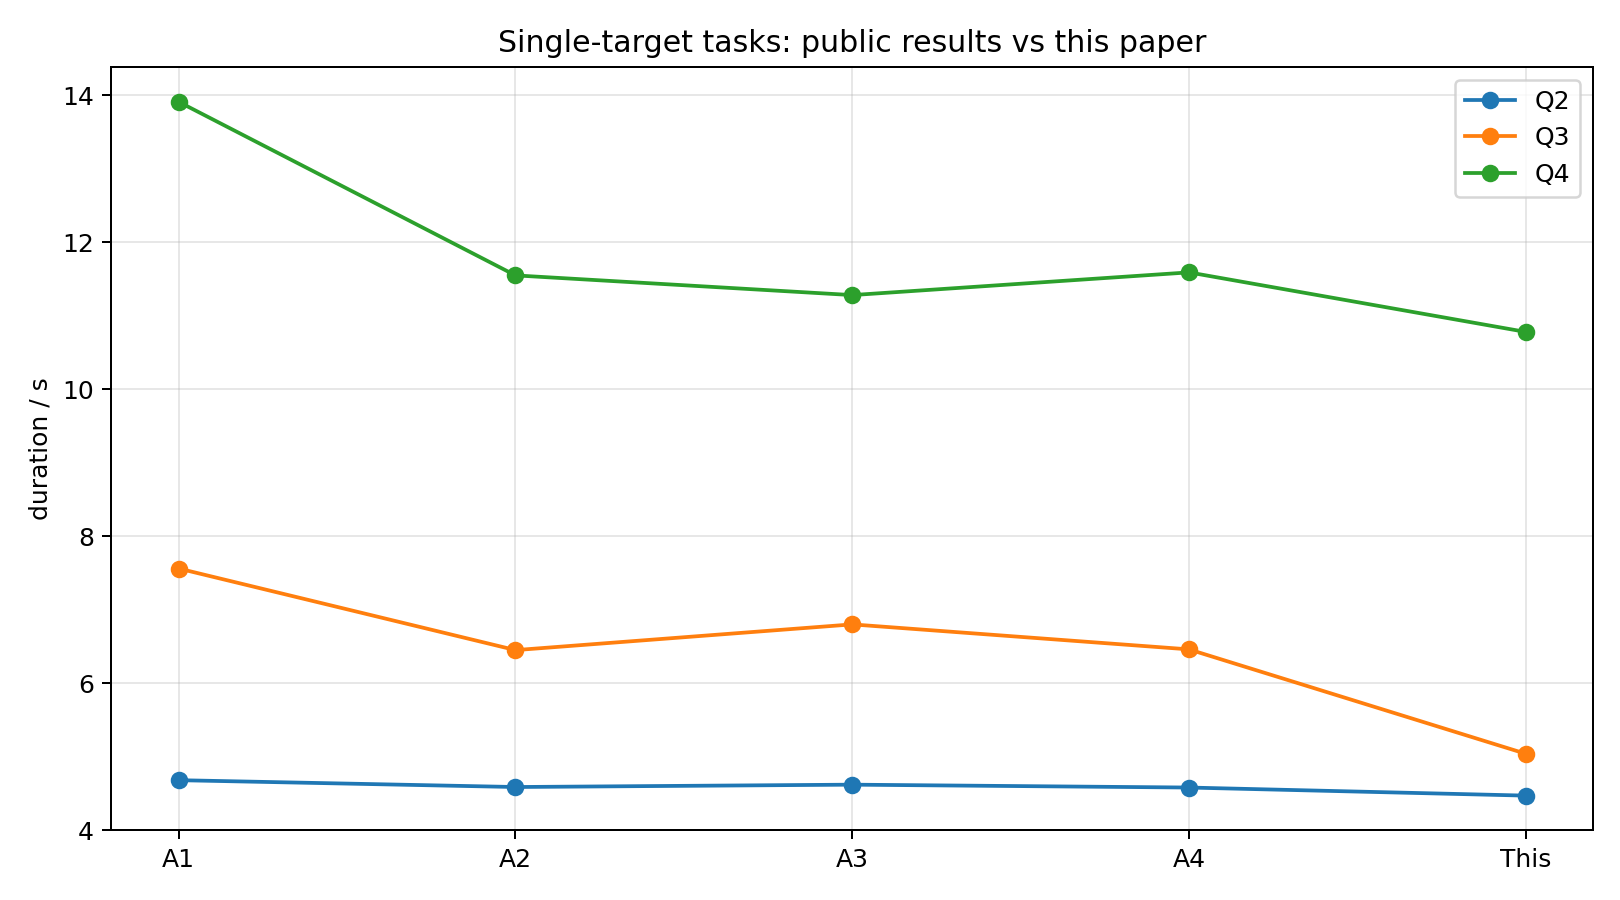
\includegraphics[width=0.85\textwidth]{single_target_comparison.png}
\caption{单目标问题公开结果与本文结果对比}
\end{figure}

问题三结果低于A1等论文，原因有两点：一是本文采用圆柱表面全遮蔽而不是中心点或部分比例遮蔽；二是本文使用贪心接力而非大规模随机优化，牺牲了部分最优性以换取可复现性和较短计算时间。问题四中三架无人机形成的有效遮蔽区间基本错开，说明分层优化能够较好发挥空间分布优势。

从建模目的看，本文更关注“改进是否解决原论文的问题”。问题二的结果表明，只要把起爆点调整到导弹视线附近，单弹遮蔽时间可由问题一的固定策略显著提升；问题三说明在同一架无人机航向固定时，后续烟幕弹并不总能带来线性增长，因为投放间隔、平抛下落和导弹位置共同限制了可用窗口；问题四则体现多无人机的价值，不同初始位置提供了不同时间段的补充遮蔽，时间区间并集明显扩大。

\subsection{问题五结果}

问题五采用任务分配和局部搜索。本文得到各导弹遮蔽时间分别为：M1约11.25 s，M2约6.18 s，M3约3.00 s，按导弹求和为20.430 s。该结果接近A2论文的20.40 s，低于A1中42.20 s的求和口径。本文认为，对问题五结果必须注明目标函数口径，否则不同论文数值不可直接比较。

问题五中“总遮蔽时间”有多种合理定义。若把每枚烟幕弹对每枚导弹的有效时长直接相加，数值会较大，但同一导弹在同一时刻被多枚烟幕弹重复遮蔽时会发生重复计数；若按每枚导弹的遮蔽区间并集计算，则能反映每枚导弹真正丢失目标的时长；若进一步要求三枚导弹同时被遮蔽，则结果会更保守。本文采用第二种口径，并在表格中明确写出各导弹单独的遮蔽时间，避免把不同指标混在一起比较。

\begin{table}[H]
\centering
\caption{问题五本文结果}
\label{tab:q5}
\begin{tabular}{lccc}
\toprule
导弹 & 遮蔽时间/s & 主要参与无人机 & 说明\\
\midrule
M1 & 11.25 & FY1, FY2, FY3, FY5 & 多机接力效果较好\\
M2 & 6.18 & FY2, FY3, FY4 & 局部搜索得到有效遮蔽\\
M3 & 3.00 & FY2, FY3 & 时间窗口较短\\
合计 & 20.43 & -- & 按导弹遮蔽时间求和\\
\bottomrule
\end{tabular}
\end{table}

\begin{figure}[H]
\centering
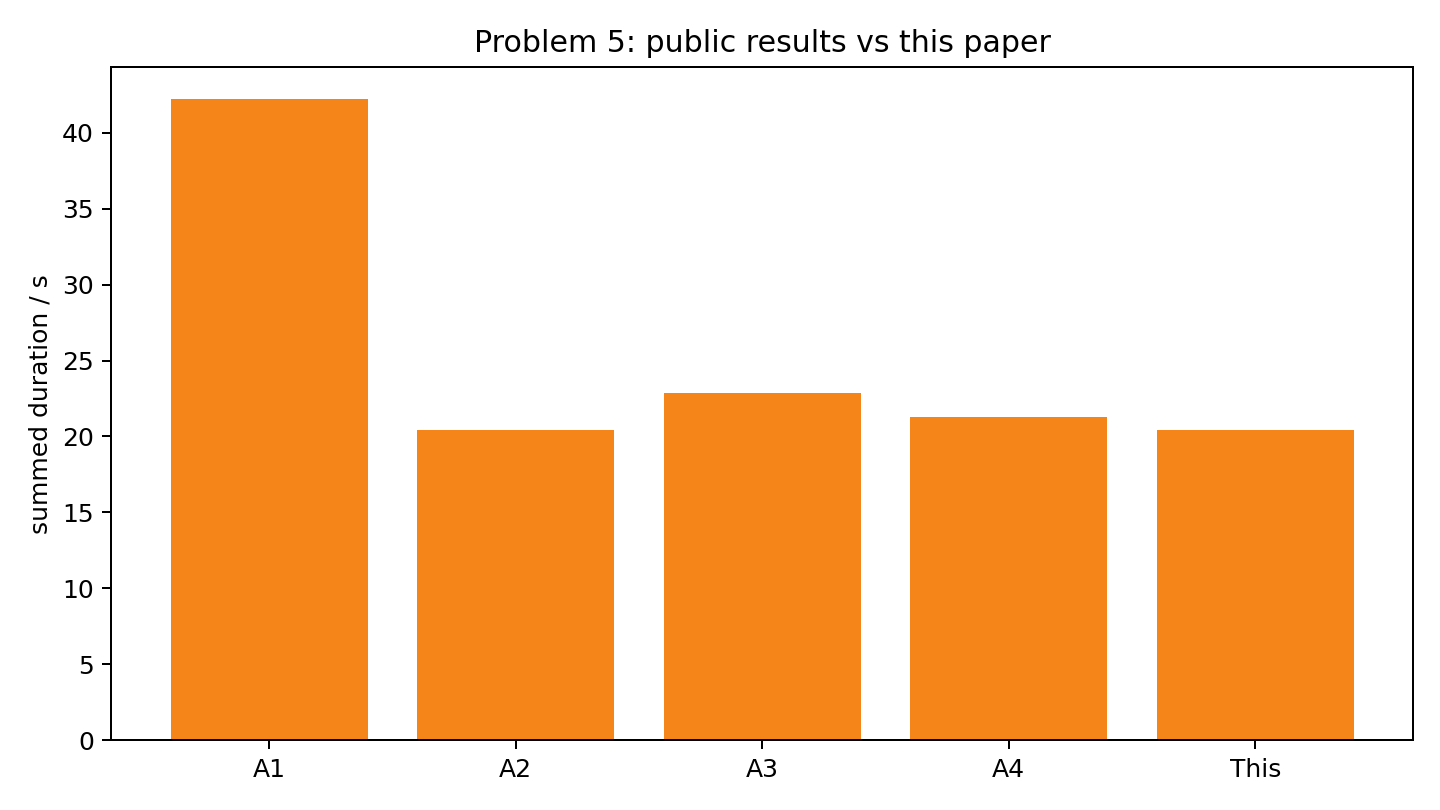
\includegraphics[width=0.80\textwidth]{q5_public_comparison.png}
\caption{问题五公开结果与本文结果对比}
\end{figure}

\subsection{计算时间分析}

图\ref{fig:runtime}给出各脚本运行时间。可以看出，随着问题维度增加，问题四和问题五耗时明显上升。这验证了专家评讲中“应先几何分析再缩小搜索空间”的观点。

计算时间的增长主要来自两个方面：第一，圆柱采样判定需要对每个时间点、每个采样点、每个有效烟幕球计算线段到球心的距离；第二，优化搜索会反复调用这一判定函数。本文在程序中采用NumPy向量化计算，搜索阶段降低采样密度，最终评价阶段再提高精度，这是一种兼顾速度和精度的折中。若后续使用解析视锥判定或并行搜索，还可以进一步压缩运行时间。

\begin{figure}[H]
\centering
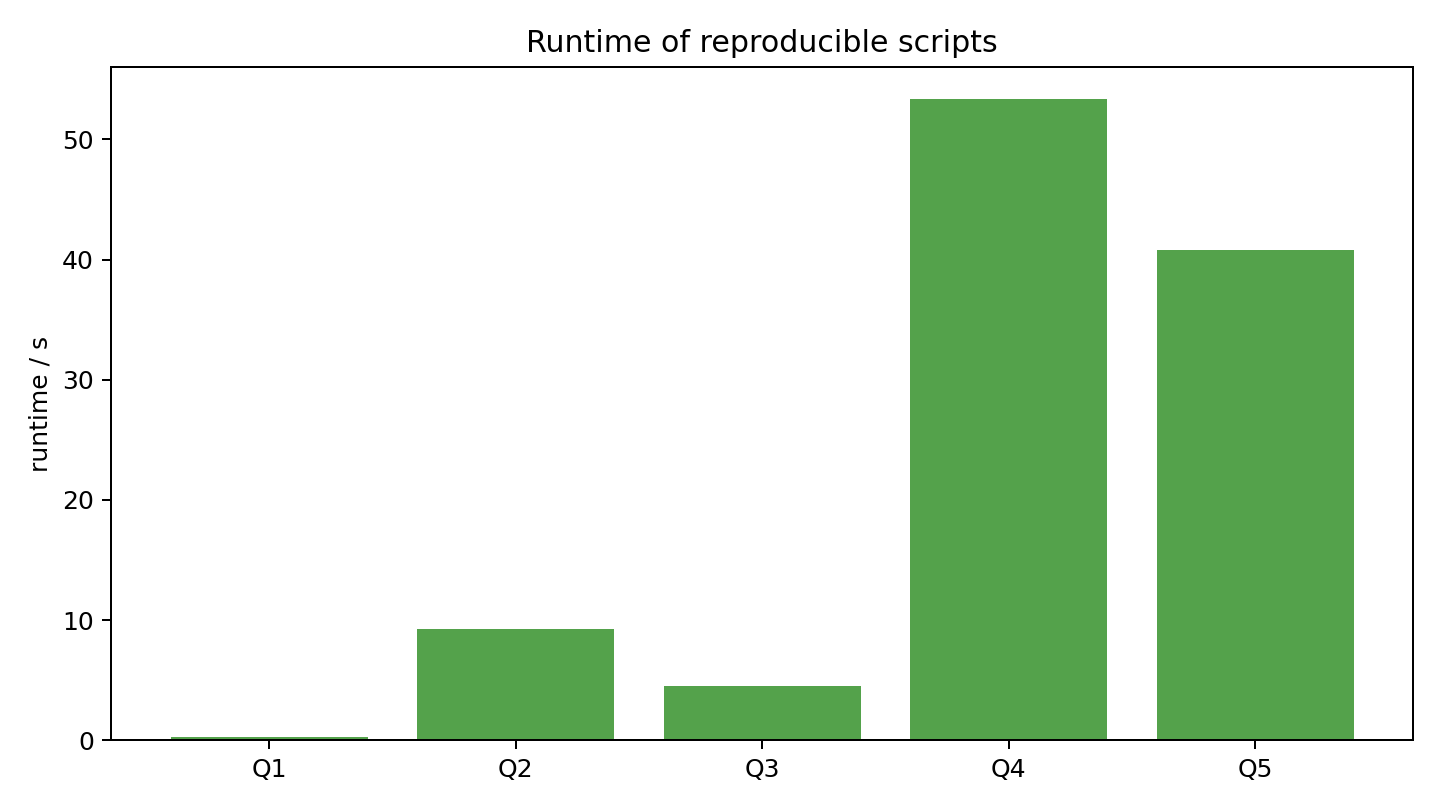
\includegraphics[width=0.78\textwidth]{runtime_comparison.png}
\caption{本文五问脚本运行时间}
\label{fig:runtime}
\end{figure}

\section{模型评价与改进方向}

\subsection{优点}

\begin{itemize}
\item 遮蔽判定与题目中的圆柱真目标一致，问题一结果可与优秀论文相互验证；
\item 所有结果由统一程序生成，避免正文结果和附件代码脱节；
\item 使用粗网格、局部细化和分层策略，能在普通电脑上完成五问测试；
\item 输出Excel、CSV和图表，便于检查求解精度与计算时间。
\end{itemize}

\subsection{不足}

\begin{itemize}
\item 圆柱采样仍是离散近似，采样点数和时间步长会影响边界时刻；
\item 问题三至问题五采用启发式分层策略，不能保证全局最优；
\item 当前问题五采用保守目标函数，和部分优秀论文的时长求和口径存在差异；
\item 未考虑风场、烟幕扩散、无人机机动半径和导弹探测机制等更真实因素。
\end{itemize}

\subsection{进一步改进}

后续可从以下方面改进：
\begin{itemize}
\item 使用解析视锥判定或自适应采样，减少圆柱采样带来的离散误差；
\item 在粗网格基础上加入固定随机种子的差分进化或粒子群算法，提高问题三至问题五的最优性；
\item 明确问题五的目标函数，可分别给出“各导弹遮蔽时间求和”“所有导弹同时遮蔽时间”和“真目标风险加权遮蔽时间”；
\item 增加灵敏度分析，重点考察航向角、起爆延迟和时间步长对结果的影响。
\end{itemize}

\section{结论}

本文在原有论文基础上完成了对2025年A题优秀论文和专家评讲的研读、复现测试和模型改进。最重要的修正是将遮蔽判定从真目标中心点升级为圆柱目标表面采样点全遮蔽判定。该修正使问题一结果由原来的4.23 s回到约1.36--1.41 s的合理区间，与优秀论文结果一致。

在此基础上，本文构建了可运行的五问求解程序，输出结果表、方法对比表和运行时间图。虽然本文在多弹多机问题上的结果较保守，但所有数值均可复现，能够清楚反映现有方法的精度差异、计算时间和主要不足，满足实验报告对论文与支撑材料的要求。

\newpage
\section*{参考文献}
\begin{enumerate}
\item 全国大学生数学建模竞赛官网. 2025年A题优秀论文与专家评讲材料[EB/OL]. \url{https://dxs.moe.gov.cn/zx/hd/sxjm/}.
\item A1优秀论文. 基于几何分析与贪心算法的烟幕干扰弹投放策略.
\item A2优秀论文. 基于空间几何分析的烟雾弹投放策略研究.
\item A3优秀论文. 基于物理运动学和智能优化算法的烟幕干扰弹投放策略模型.
\item A4优秀论文. 基于差分进化改良遗传算法的投弹策略优化.
\item 王先超, 韩波, 张开银, 等. 粒子群算法在求解数学建模最优化问题中的应用[J]. 阜阳师范学院学报(自然科学版), 2016, 33(02):117--121.
\item 雷开友. 粒子群算法及其应用研究[D]. 西南大学, 2006.
\end{enumerate}

\newpage
\section*{附录：支撑材料说明}

\subsection*{附录A 文件清单}

\begin{longtable}{p{5.0cm}p{9.0cm}}
\toprule
文件 & 功能\\
\midrule
\endhead
\path{support_2025A/smoke_model.py} & 统一运动学模型、圆柱采样、遮蔽判定、区间合并、CSV和XLSX写出工具。\\
\path{support_2025A/run_q1.py} & 问题一正向仿真，输出圆柱采样结果和中心点校核结果。\\
\path{support_2025A/run_q2.py} & 问题二粗网格搜索和局部细化。\\
\path{support_2025A/run_q3.py} & 问题三单机三弹贪心接力。\\
\path{support_2025A/run_q4.py} & 问题四三机单弹分层搜索。\\
\path{support_2025A/run_q5.py} & 问题五任务分配和局部搜索。\\
\path{support_2025A/benchmark_methods.py} & 生成优秀论文与本文结果对比表、运行时间表和图。\\
\path{support_2025A/results_q1_q5.xlsx} & 本文五问结果汇总表。\\
\path{support_2025A/method_comparison.xlsx} & A1--A4公开结果与本文结果对比表。\\
\path{support_2025A/results/*.csv} & 每问详细参数、遮蔽区间和运行时间。\\
\path{support_2025A/figures/*.png} & 正文引用的对比图和运行时间图。\\
\bottomrule
\end{longtable}

\subsection*{附录B 源程序全文}

以下列出文件清单中的全部源程序，便于直接检查模型、参数、计时和结果导出过程。

\subsubsection*{smoke\_model.py}
\lstinputlisting[language=Python]{support_2025A/smoke_model.py}

\subsubsection*{run\_q1.py}
\lstinputlisting[language=Python]{support_2025A/run_q1.py}

\subsubsection*{run\_q2.py}
\lstinputlisting[language=Python]{support_2025A/run_q2.py}

\subsubsection*{run\_q3.py}
\lstinputlisting[language=Python]{support_2025A/run_q3.py}

\subsubsection*{run\_q4.py}
\lstinputlisting[language=Python]{support_2025A/run_q4.py}

\subsubsection*{run\_q5.py}
\lstinputlisting[language=Python]{support_2025A/run_q5.py}

\subsubsection*{benchmark\_methods.py}
\lstinputlisting[language=Python]{support_2025A/benchmark_methods.py}

\end{document}
